% %This is a very basic article template.
% %There is just one section and two subsections.
\documentclass[a4paper,12pt]{article} % classe "article", papier a4 et police de
% 11pt

\usepackage[utf8]{inputenc} \usepackage[T1]{fontenc}
\usepackage{cite}
\usepackage{mathptmx}
\usepackage[english]{babel}
\usepackage{amsmath,amsfonts,amsthm,amssymb}
\usepackage{graphicx}
\usepackage{multicol}
\usepackage{abstract}
\usepackage[center,labelfont=bf]{caption}
\usepackage{tocloft}
\usepackage{indentfirst}

\usepackage[margin=25mm]{geometry}


\title{
\vspace{-50pt}
\hfill\large{\textbf{P1-050}}\\[1cm] \textbf{\large{Charge and Current Transport
in Open Field Lines Turbulence}\\
\normalsize{Influence of Plasma-Surface Boundary Conditions}}}

\author{\normalsize{\textbf{R. Futtersack}\textsuperscript{ab*}, P.
Tamain\textsuperscript{a}, G. Hagelaar\textsuperscript{b},
 Ph. Ghendrih\textsuperscript{a}, 
 %J.P. Boeuf\textsuperscript{b}, 
 A. Simonin\textsuperscript{a}}\\
\small{\emph{\textsuperscript{a}CEA, IRFM}
\emph{F-13108 St. Paul-lez-Durance, France}}\\
\small{\emph{\textsuperscript{b}Universite Paul Sabatier Toulouse - LAPLACE-}
\emph{118 route de Narbonne, F-31062 Toulouse cedex 9}}}
\date{}

\linespread{1.6}

\begin{document}
\linespread{1}
\maketitle

\thispagestyle{empty}
\linespread{1.6}
\renewcommand{\absnamepos}{flushleft}
\renewcommand{\abstractnamefont}{\normalfont\textbf}
\renewcommand{\abstracttextfont}{\normalsize}

\cftpagenumbersoff{figure}
\renewcommand{\cftdotsep}{\cftnodots}
\renewcommand{\cftfigpresnum}{\textbf{Figure~}}
\renewcommand{\cftfigaftersnum}{:}
\cftsetindents{figure}{0em}{6em}
\renewcommand{\cftbeforefigskip}{1em}


\setlength{\absparindent}{0cm}
\setlength{\absparsep}{0cm}
\setlength{\absleftindent}{0pt}
\setlength{\absrightindent}{0pt}

\begin{abstract}
We investigate the impact of both parallel and transverse boundary conditions on the current and charge transport
in open field line systems using the TOKAM2D code, which solves a minimal model for interchange turbulence. 
Various limit test cases are discussed and analyzed. In the parallel direction,
the sheath conductivity is found to play an essential role in the stabilization of large-scale potential structures,
leading to the formation of transport channel or transport barrier respectively for an insulating end wall or a wall 
with an enhanced sheath conductivity. On another hand, the addition of transverse boundary conditions intrinsically changes
the transport characteristics, influencing both radial profiles and probability density functions. It underlines that 
in some cases a detailed description of the plasma-wall interaction process is required to get a proper description of
 the current loop pattern that determines electrostatic turbulent transport.\\
\hrule
\end{abstract}

\newenvironment{correct}%
{\noindent\ignorespaces\linespread{1}}%
{}

\begin{correct}
\emph{PACS}: 52.35.Ra, 52.65.Kj, 52.25.Xz, 05.45.-a\\
\emph{PSI-20 keywords}: Cross-field transport, Fluctuation \& turbulence\\
\emph{*Corresponding author address}: CEA Cadarache, F-13108
Saint-Paul-lez-Durance, France.\\
\emph{*Corresponding author E-mail}:  romain.futtersack@cea.fr\\
\emph{Presenting author}: R. Futtersack\\
\emph{Presenting author e-mail}: romain.futtersack@cea.fr\\
\end{correct}
\linespread{1.6}
\newpage
\begin{section}{Introduction}
The presence of a physical object in the Scrape-of-Layer (SOL) of a tokamak is crucial in the edge plasma physics.
Magnetic field lines are intercepted by a solid surface, which then act as a perfect particle sink. Moreover, 
in these open field line systems, transverse transport mainly results from a plasma turbulence governed 
by self-sustained electromagnetic fields generated by electric polarization or electric currents~\cite{Zweben}.
At low enough plasma pressure, the electrostatic turbulence results from the
competition between the drive due to the transverse diamagnetic current (vertical charge separation) and
damping by parallel currents. The polarization current allows to close the current loops by controlling the 
transverse transport of the electrostatic potential. This mechanism is known as interchange turbulence and 
is thought to dominate perpendicular transport in the SOL of tokamaks.
 
Charge transport through current loops thus appears as a major element
of plasma confinement in open field line systems.
Modeling and understanding these properties then require an appropriate description 
of the electric current flowing between the plasma and the wall elements. In the parallel direction, one
can consider that the sheath physics provide a reliable description backed up by solid theoretical 
considerations~\cite{Riemann,Stangeby}. In the transverse direction, the physics of the plasma-wall boundary is
more complex to handle, since no equivalent of the Bohm criterion has been derived. 

In this paper, we study how the circulation of current can impact the transport characteristics
through the parallel and transverse boundary conditions modification. 
The paper is organized as follows: in section 1 we describe the physical 
model used for the SOL interchange turbulence. Then we analyze the effect of changing parallel and transverse 
boundary conditions respectively in section 2 and 3. Finally, discussion of the results and their implications 
for SOL cross-field transport are found in section 4.
\end{section}
\begin{section}{TOKAM2D, a minimal model for SOL interchange turbulence}
In the last two decades, 2D models have been developed in order to capture and understand most of the essential
characteristics of SOL turbulence observed in experiments.
As a common point, most of them rely on an interchange model ~\cite{Nedospasov,Garbet,Esel,Bisai}. The following work relies 
on the TOKAM2D model which solves the current 
balance equation $\text{~}\vec{\nabla}\cdot\vec{j}=0\text{~}$ in conjunction with the 
continuity equation $\text{~}d_tn=S\text{~}$ to determine the evolution of the electrostatic potential and
density fields~\cite{Sarazin}. The perpendicular turbulent
transport is described in term of drifts (electric, diamagnetic and polarization) and is driven by an
incoming particle flux instead of a density gradient, which give rise to an avalanche-like dynamics characterized
by profile relaxation and strong outwards bursts of density~\cite{Sarazin}. The parallel boundary conditions, 
derived from the Bohm 
criterion, appear through source terms after the integration of the equations along the parallel direction on the basis
of the flute hypothesis, which ensures the reduction of the model to two dimensions.
Assuming the plasma is isothermal with $T_i<<T_e$, the system is then reduced to~\cite{Sarazin}:
\begin{align}
\label{eqDensity}\partial_tN+\left[\phi,N\right]&=-\sigma_N N e^{\Lambda-\phi}+D\nabla^2_\perp N +S_N\\
\label{eqCurrent}\partial_t\nabla^2_\perp \phi+\left[\phi,\nabla^2_\perp \phi\right]&=\sigma_\phi(1-e^{\Lambda-\phi})-g\partial_y\log(N)+\nu\nabla^4_\perp \phi
\end{align}
with two fields, the normalized density $N=n_e/n_0$ and the normalized electric potential $\phi=eU/T_e$, taken
with the wall potential as reference, $U$ being the electric potential, $e$ the electric charge and $T_e$ the 
electron temperature. Note that $n_0$ is an arbitrary reference density (the system is independent of the value of $n_0$).
Time is normalized to the inverse of $\omega_c=eB_0/m_i$ the ion cyclotron frequency while space is normalized 
to the Larmor radius $\rho_L=c_s/\omega_c$ where $c_s=\sqrt{T_e/m_i}$ is the acoustic velocity. 
The Poisson brackets derive from the electric drift flux divergence and are defined by 
$[\phi,f]=\vec{b}\cdot(\vec{\nabla} \phi\times\vec{\nabla} f)$, with $\vec{b}$ the unit vector in the direction 
of the magnetic field. $\sigma_N$ and $\sigma_\phi$ characterize the sheath losses ($\sigma_N$ for density 
and $\sigma_\phi$ for current) in order to control the parallel fluxes. The divergence of the diamagnetic 
current, driving the interchange instability, is found to be proportional to a curvature coefficient $g$. 
The floating potential $\Lambda=0.5\cdot\log(m_i/(2\pi m_e))$ corresponds to the equilibrium 
potential canceling out the sheath current. $S_N$ (the source term mimicking an incoming particle flux 
from the plasma core) is a Gaussian centered on the first third of the domain, and 
is defined by $S_N=S_0\cdot e^{-\frac{(x-x_S)^2}{L_S}}$. 
Finally, $D$ and $\nu$ are normalized to the 
Bohm coefficient $D_B=T_e/eB_0$, and account for transport processes which are not included in the model such as 
collisional transport. Their main effect is to stabilize the simulations by the damping of small scales. 

Equations (\ref{eqDensity}) and (\ref{eqCurrent}) are solved in 2D slab geometry: 
$x=r/\rho_L$ with $r$ the minor radius and $y=r\theta/\rho_L$ with $\theta$ the poloidal angle.
The initial version of the TOKAM2D code was developed by using bi-periodical transverse boundary conditions.
For the following study, an upgraded version of the code was developed to 
include and assess the impact of non-periodical transverse boundary conditions. In both cases, the source region 
(of width $L_S$) separates the domain between an unstable gradient region 
(unfavorable gradient with respect to the interchange instability) located on the right hand side of the source
along the x-axis and a stable gradient region located on the left hand side.

In this paper, we focus mainly on the impact of boundary conditions for charge fluxes. We will in particular 
analyze their impact in terms of charge transport by the three currents involved in the charge 
balance Eq.~(\ref{eqCurrent}), \emph{ie.} the parallel current, the diamagnetic current and the polarization current, 
whose divergence are the following:
$$\vec{\nabla}\cdot\left(\vec{j}_\parallel\right)=\sigma_\phi (1-e^{\Lambda-\phi})\text{~~~~~~~}
  \vec{\nabla}\cdot\left(\vec{j}_{dia}\right)=-g\partial_y\log(N)\text{~~~~~~~}
  \vec{\nabla}\cdot\left(\vec{j}_{pol}\right)=-\partial_t\nabla^2_\perp \phi-\left[\phi,\nabla^2_\perp \phi\right]
  +\nu\nabla^4_\perp \phi$$
Note first of all that the sum of the current divergences involved in the model is equal to zero by construction, 
and that the diffusive current term is taken into account as a component of the polarization current divergence. 
However, its contribution is negligible compared to the other terms (of the order of 1\%).

Unless explicitly stated, the simulations studied in this paper were run with the following set of parameters : 
$g=6\cdot 10^{-4}$, $\sigma_N=\sigma_\phi=10^{-5}$, $D=\nu=10^{-3}$ with a simulation box of size 
$L_x=L_y=256\text{~}\rho_L$ discretized 
by $N_x=N_y=256$ grid points. 
Expect in section 3, where the sheath conductivities $\sigma_N$ and $\sigma_\phi$ are locally modified in a stripe in the
middle of the unstable region, the model parameters are taken uniform in the whole domain.
\end{section}

\begin{section}{Impact of sheath current boundary condition on turbulent transport}
As previously mentioned, the current flow parallel to the magnetic field is governed by sheath physics and the Bohm 
criterion. The electron outflow is then given by $\nonumber -\sigma_N N e^{\Lambda-\phi}$
and the charge outflows follows $\nonumber \sigma_\phi(1-e^{\Lambda-\phi})$.  This boundary condition on current
regulates the electrostatic potential and damps electrostatic fluctuations, by dragging back the plasma 
potential to the floating potential. It has already been proved that a local polarization of the wall 
(mimicking a Langmuir probe)
can influence the plasma density through its impact on the charge balance~\cite{Ghendrih} while recent experiments 
on linear devices demonstrated that changes in the electrical conductivity of the wall at the end of 
field lines~\cite{UCSD} impact the global transport. 
Such experiments can be studied with the TOKAM2D code through the control of the parallel charge fluxes. 
This can be made by zeroing (insulating the wall) or enhancing the sheath conductivity ($\sigma_\phi$) on 
a radially localized stripe around $x=\frac{3}{4}\text{~}Lx$. Simulations are run under periodic transverse boundary conditions.

\textbf{Insulating wall.}
In the insulated area the parallel current is totally canceled ($\sigma_\phi=0$) and we drop the potential dependence
of the density loss term : $\sigma_N N e^{\Lambda-\phi}\rightarrow\sigma_N N$. The gradient of the mean density radial profile (presented in fig. \ref{profileN}) is 
locally impacted around the location of the stripe by the parallel boundary condition ; it slightly steepens 
in the near region before flattening
which results from an enhancement of the radial transport due to the formation of vortices around large potential 
structures. These structures grow up as expected 
from the dispersion relation resulting from the linear study (which predicts the stabilization of large-scale 
potential fluctuations by the sheath conductivity~\cite{Sarazin}), until reaching a size of the order of the 
insulated stripe width.
Figure \ref{FFTyPhi} clearly shows this increase of large modes, with an amplification of the $k_y<0.1\cdot\rho_L^{-1}$ 
wave vectors
 a decade higher than in the reference case, corresponding to the typical size of these structures. They also have 
a resilient behavior with a longer lifetime and a slower motion, as one can observe in figure \ref{FFTtW} where 
an increase of low frequencies is evidenced inside the insulating stripe. In figure~\ref{PHI} we see that long-lived transport channels are then established between 
these large structures, connecting both sides of the insulated stripe. Moreover, in the probability distribution 
function of density presented in figure 
\ref{pdfN}, the shifting of the skewness points out the impact on the turbulent transport statistics. 

\textbf{Enhanced parallel current losses.} We now consider the case where the stripe favors outgoing parallel 
currents, which is done by increasing locally the sheath conductivity to $\sigma_\phi=10^{-4}$. As can be expected, 
the results show a phenomenology that is opposite.
The area with enhanced sheath conductivity prevents the formation of large-scale electrostatic potential 
structures, damping small $k_y$ wave vectors (figure \ref{FFTyPhi}) and driving a strong barrier for the turbulent 
transport. The mean equilibrium state presented in figure \ref{profileN} shows the consequent rise of mean density 
in front of the barrier. 
One can also notices a change in the dynamics of the system: Figure \ref{currentDiv1}
shows the time evolution of the local current divergence in the conductive strip, comparing the reference simulation 
with that with enhanced $\sigma_\phi$. In the reference case, 
we clearly notice two main dynamics: the parallel current divergence evolves on a slow time scale (potential fluctuations)
while diamagnetic and polarization currents divergences present a faster behavior. 
In the case with increased sheath conductivity, the weight of the parallel current in the current balance equation 
is enhanced so that it imposes its slower dynamics to the perpendicular currents. 
The temporal spectrum of vorticity in the conductive stripe (see figure \ref{FFTtW}) 
also shows a strong damping of high frequency components, pointing out the modification in the polarization current 
dynamics.
\end{section}

\begin{section}{Changes in the transverse boundary conditions}
In contrast with the Bohm boundary conditions, which have been derived for 
non-grazing incidence~\cite{Stangeby}, there is no well-based theory to model the plasma-wall interaction 
in the transverse direction. 
Moreover, experimental studies show the Bohm theory fails in such cases~\cite{Krasheninnikova}. 
This question is not only important for the SOL of tokamaks but also in other experiments, like in ion sources 
where the polarized wall required to extract negative ions~\cite{Hagelaar} can impact 
the transport in an unconventional way. 
The lack of available physical model to describe this interaction makes that arbitrary simple boundary conditions 
are commonly used (like in the periodical TOKAM2D). Such choices may have consequences on simulation results, 
and one has to measure their influence on the turbulent transport main characteristics.
In order analyze this issue, we compare here the three most used techniques, namely (1) the periodic (the reference 
case from section 3), (2) the Neumann boundary conditions $\partial_{\vec{n}}\phi(x)= f(x)$ and (3) the 
Dirichlet $\phi_\Omega = \phi_{wall}$. 

\textbf{Von Neumann boundary conditions.} We first consider a zero-gradient condition for the
density and potential fields, while perfectly absorbing boundary conditions are used for the vorticity 
($W=0$ outside the computational domain). 
In comparison with the standard bi-periodical case, several effects can be observed in figure~\ref{profileN2}: 
in the unfavorable curvature region with respect to the interchange instability~\cite{Sarazin} ($x>x_{S}$, \emph{ie.} 
where $\vec{\nabla B}\cdot\vec{\nabla N}>0$), the absorption of vorticity
by the wall is responsible for the damping of potential fluctuations near the border, quenching the turbulence 
and consequently reducing the current transport while the mean density increases.
Note that the stable region ($x<x_S$) presents an e-folding length of density consequently 
reduced while the potential equals to 
the floating potential. This is due to the fact that this area is not fed anymore in particle or current flows 
by turbulent transport through the periodic boundary conditions. The equilibrium is then 
established only by the balance between the parallel particle loss and the dissipative terms. The change in the 
transverse boundary conditions also impacts the turbulence characteristics away from the wall. 
This is illustrated in Fig.~\ref{pdfN2} where the probability distribution function of the density fluctuations 
at mid-way between the source and the wall on the unstable gradient side is plotted and compared with 
the bi-periodic reference. 
One can observe a change of the wings of the PDF towards a higher skewness, reducing the number small amplitude events 
and increasing the occurrence of large events.

\textbf{Dirichlet boundary conditions.} For this second case, we use the Dirichlet boundary condition 
for potential, setting it to the floating potential: this option is often chosen as it is the most simple to implement. 
Our simulations show that it obviously leads to significant changes near the wall as can be seen in figure \ref{profileN2}. 
As the potential is poloidally constant, radial drift fluxes which depend on the poloidal gradient of potential,
are null on the boundary, shutting off all radial transport. 
Density can not be evacuated anymore through the transverse direction and accumulates up to the wall.
More interestingly, one can observe an impact of the change of boundary conditions in figure \ref{pdfN2} 
which shows the PDF of density fluctuations at the midpoint of the unstable region (between the source and the wall). 
As in the Neumann boundary conditions case, a modification of the turbulence characteristics even at such distance 
from the wall is observed, in the direction of a largest skewness of the density PDF. 
\end{section}

\begin{section}{Conclusions} 
In this work, we showed that changes in the circulation of currents in a 2D model of SOL interchange turbulence 
dramatically impacts turbulence and the related transport. An enhancement of the parallel current through the 
sheath boundary condition stabilizes large scale potential structures and consequently reduces radial transport, 
leading to the formation of a local transport barrier. On the contrary, blocking the parallel current circulation by
including insulating wall boundary conditions on both sides of the magnetic field lines generates large long-lived
electrostatic potential vertices, leading to an enhancement of radial transport and a flattening of the density profile. 
The impact of boundary conditions on the plasma potential (hence on currents) in the perpendicular direction was 
also studied. Although the impact on profiles is much less dramatic than when changing the circulation of parallel 
currents, we showed that turbulence characteristics can be influenced by perpendicular boundary conditions even away 
from the location where they are applied.

This way, the circulation of currents, and in particular the constraints imposed to it by boundary conditions, appears as 
a key point of SOL turbulent transport physics. The plasma develops complex current loops through the sheath and the 
wall material which cannot be overlooked when modeling SOL turbulence. In the case of perpendicular boundary conditions, 
\emph{ie.} the case of a wall tangential or nearly tangential to the magnetic field, modelers are often reduced to 
the use of simple ideal boundary conditions (Dirichlet, Neumann) due to the absence of a well-defined model such as the 
Bohm theory (Bohm-Chodurah for an oblic incidence). One must be aware that this choice is not consequence-less on the 
plasma turbulence, highlighting the need for a theory comparable to the Bohm's one for transverse conditions.
\end{section}
\section*{Acknowledgments}
This work, supported by the European Communities under the contract of
Association between EURATOM and CEA, was carried out within the
framework of the European Fusion Development Agreement and has been financially supported by the French National Research 
Agency (ANR), projects ITER-NIS (BLAN08-2\_310122) and METRIS (ANR-11-JS09-008). The views and
opinions expressed herein do not necessarily reflect those of the
European Commission.
\newpage

\begin{thebibliography}{1}

\bibitem{Zweben} S. J. Zweben et al, {\em Plasma Phys. Control. Fusion 49} (2007), S1
\bibitem{Riemann} K.-U. Riemann, {\em J. Phys. D: Appl. Phys. 24} (1991), 493
\bibitem{Stangeby} P. C. Stangeby and A. V. Chankin, {\em Phys. Plasma 2} (1995), 707
\bibitem{Nedospasov} A.V. Nedospavov, {\em Sov. J. Plasma Phys. 15} (1989), 659
\bibitem{Garbet} X. Garbet et al, {\em Nucl. Fusion 31} (1991), 967
\bibitem{Esel} O. E. Garcia et al, {\em Plasma Phys. Control. Fusion 45} (2003), 919
\bibitem{Bisai} N. Bisai, {\em Phys. Plasma 12} (2005), 072520
\bibitem{Sarazin} Y. Sarazin, Ph. Ghendrih, {\em Phys. Plasma 5} (1998), 4214
\bibitem{Ghendrih} Ph. Ghendrih et al, {\em Nucl. Fusion 43} (2003), 1013
\bibitem{UCSD} G. Tynan, private communication
\bibitem{Krasheninnikova} N. S. Krasheninnikova, X. Tang and V. S. Roytershteyn, {\em Phys. Plasma 17} (2010), 057103
\bibitem{Hagelaar} G. J. M. Hagelaar and al, {\em Plasma Sources Sci. Technol. 20} (2011), 015001

\end{thebibliography}
\newpage

\listoffigures
\newpage
\thispagestyle{empty}

\section*{Figures}
\center
\begin{figure}[h!]
\center
\caption[Comparison of mean radial profile of SOL density. 
		$\nabla \bar{n}$ is locally impacted around the location of the stripe where the sheath 
		conductivity was changed.]{}
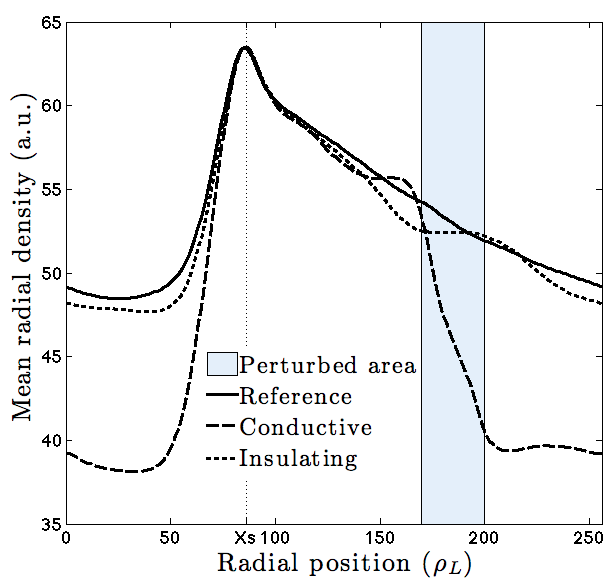
\includegraphics[height=60mm,width=75mm]{figures/FigurePSI2012_1_P1-50_Futtersack.png}
\label{profileN}
\end{figure}

\thispagestyle{empty}

\begin{figure}[h!]
\center
\caption[Spatial Fourier transform of potential at the center of the stripe where the sheath current boundary 
conditions are modified.]{}
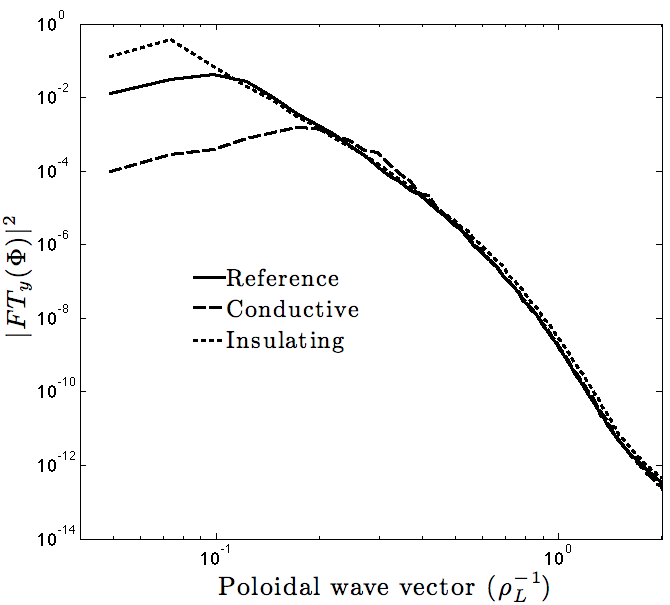
\includegraphics[height=60mm,width=75mm]{figures/FigurePSI2012_2_P1-50_Futtersack.png}
\label{FFTyPhi}
\end{figure}

\thispagestyle{empty}



\begin{figure}[h!]
\center
\caption[Temporal spectrum of vorticity $\nabla^2\phi=W$ at the center of the stripe of modified sheath conductivity.]{}
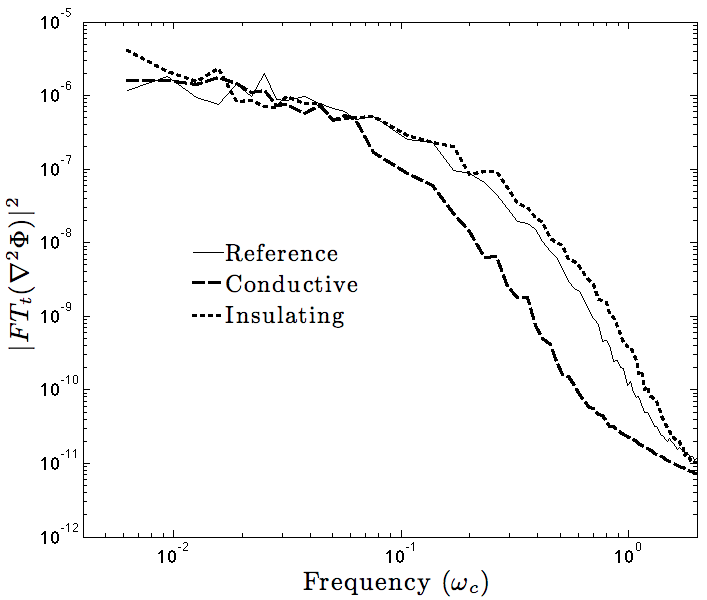
\includegraphics[height=60mm,width=75mm]{figures/FigurePSI2012_3_P1-50_Futtersack.png}
\label{FFTtW}
\end{figure}


\thispagestyle{empty}

\begin{figure}[h!]
\center
\caption[2D snapshot of the electrostatic potential for the insulating case. Arrows show the direction of the 
$\vec{E}\times \vec{B}$
 drift between the potential structures. The electrostatic potential is expressed in $Te/e$ unit.]{}
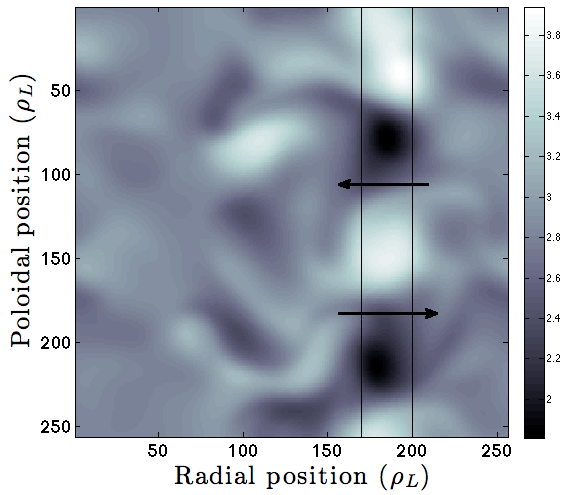
\includegraphics[height=60mm,width=75mm]{figures/FigurePSI2012_4_P1-50_Futtersack.png}
\label{PHI}
\end{figure}


\thispagestyle{empty}

\begin{figure}[h!]
\center
\caption[PDF of density fluctuations at the center of the strip where the sheath current boundary conditions are modified. The scale of the x axis is the density fluctuations normalized to 
	the RMS value.]{}
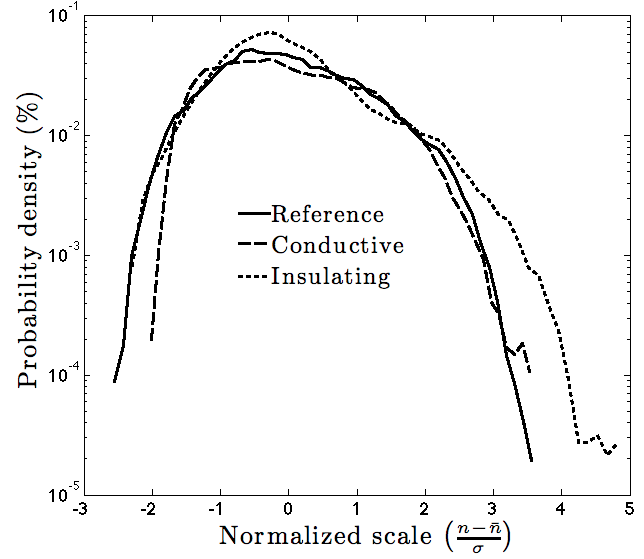
\includegraphics[height=60mm,width=75mm]{figures/FigurePSI2012_5_P1-50_Futtersack.png}
\label{pdfN}
\end{figure}

\thispagestyle{empty}

\begin{figure}[h!]
\center
\caption[Contribution of the three main currents to the current balance equation as a function of time for the reference case (left) and for the enhanced sheath conductivity case at the center of the stripe of modified sheath conductivity.]{}
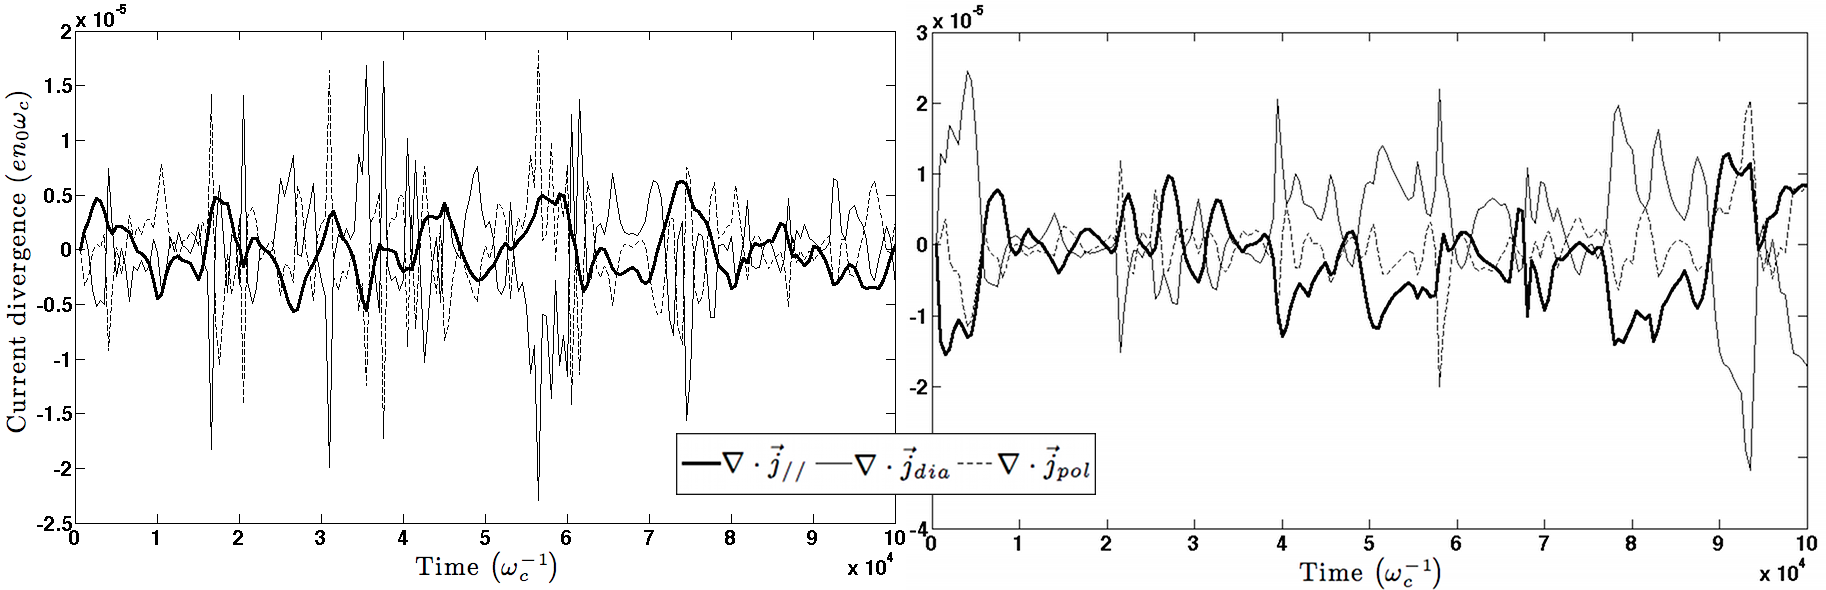
\includegraphics[height=60mm,width=160mm]{figures/FigurePSI2012_6_P1-50_Futtersack.png}
\label{currentDiv1}
\end{figure}


\thispagestyle{empty}



\begin{figure}[h!]
\center
\caption[Mean radial profile of SOL density. The loss of periodicity leads to the rise in $\bar{n}$.]{}
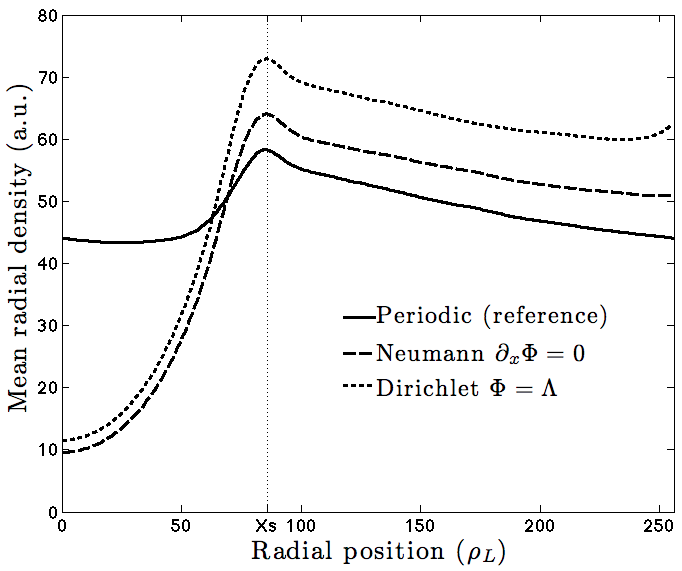
\includegraphics[height=60mm,width=75mm]{figures/FigurePSI2012_7_P1-50_Futtersack.png}
\label{profileN2}
\end{figure}

\thispagestyle{empty}

\begin{figure}[h!]
\center
\caption[PDF of density at a midpoint between the center of the source ($x=x_S$) and the wall. The three cases studied 
in section 4 (bi-periodic, Neumann and Dirichlet boundary conditions) are compared.]{}
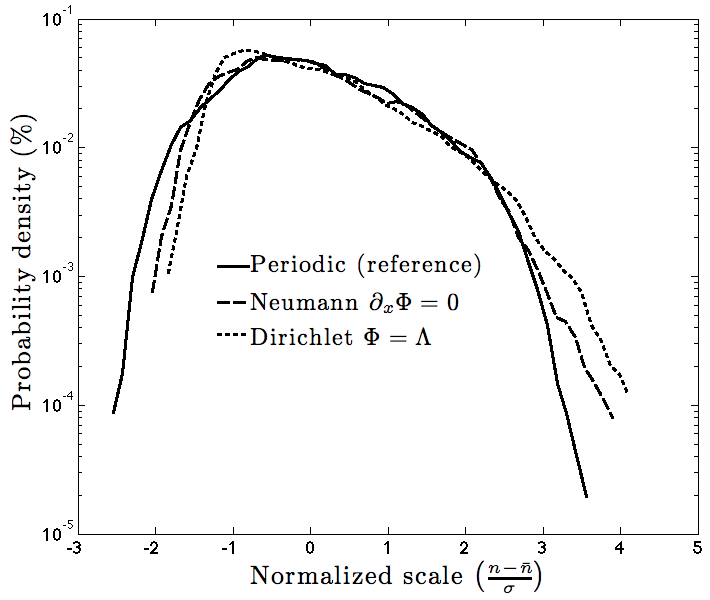
\includegraphics[height=60mm,width=75mm]{figures/FigurePSI2012_8_P1-50_Futtersack.png}
\label{pdfN2}
\end{figure}
\end{document}
